\documentclass{article}%, handout
\usepackage{tikz}
\definecolor{backgroundColor}{HTML}{2D2D2D}
\usetikzlibrary{arrows}
\usetikzlibrary{backgrounds}
\begin{document}
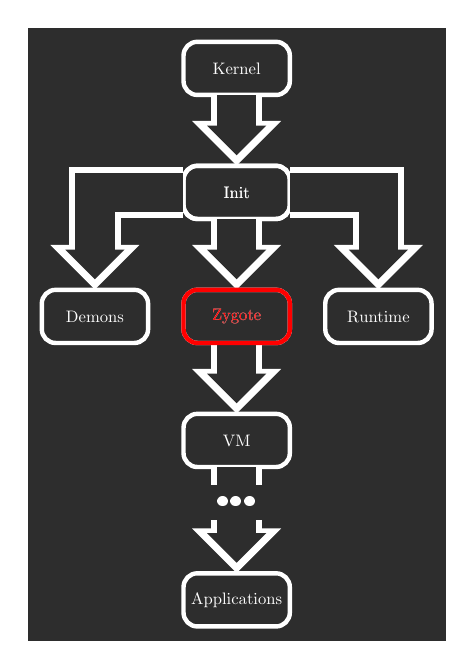
\begin{tikzpicture}[scale=0.45, every node/.style={scale=0.6},show background rectangle,
    background rectangle/.style={fill=backgroundColor},color=white,]
    \tikzstyle{myarrows}=[thick, line width=1.7mm,-open triangle 90,
    postaction={draw, line width=6.5mm, shorten >=4mm, -},
    postaction={draw, backgroundColor, shorten >= 1.3mm, -triangle 90, line width=1mm},
    postaction={draw, line width=5mm, backgroundColor, shorten >= 4mm, -}]
    
\draw [ultra thick, rounded corners=5] (0,0) rectangle node{
Kernel
} (3,-1.5);
\node[inner sep=0,minimum size=0] at (1.5,-1.5) (K) {}; % invisible node
\draw [ultra thick, rounded corners=5] (0,-3.5) rectangle node{
Init
} (3,-5);
\node[inner sep=0,minimum size=0] at (1.5,-3.5) (I0) {}; % invisible node
\node[inner sep=0,minimum size=0] at (0,-4.25) (I1) {}; % invisible node
\node[inner sep=0,minimum size=0] at (3,-4.25) (I2) {}; % invisible node
\node[inner sep=0,minimum size=0] at (1.5,-5) (II) {}; % invisible node

\draw [ultra thick, rounded corners=5] (0,-3.5) rectangle node{
Init
} (3,-5);

\draw[myarrows] (K) to (I0);

\node[inner sep=0,minimum size=0] at (1.5,-3.5) (Z0) {}; % invisible node
\node[inner sep=0,minimum size=0] at (1.5,-8.5) (Z1) {}; % invisible node
\onslide<1-5|handout:0>{\draw [ultra thick, rounded corners=5] (0,-7) rectangle node{
Zygote
} (3,-8.5);}

\node[inner sep=0,minimum size=0] at (1.5,-7) (Z0) {}; % invisible node
\draw[myarrows] (II) to (Z0);


\draw [ultra thick, rounded corners=5] (-4,-7) rectangle node{
Demons
} (-1,-8.5);
\node[inner sep=0,minimum size=0] at (-2.5,-7) (D) {}; % invisible node
\draw[myarrows] (I1) -| (D);

\draw [ultra thick, rounded corners=5] (4,-7) rectangle node{
Runtime
} (7,-8.5);
\node[inner sep=0,minimum size=0] at (5.5,-7) (R) {}; % invisible node
\draw[myarrows] (I2) -| (R);

\node[inner sep=0,minimum size=0] at (1.5,-10.5) (VM0) {}; % invisible node
\node[inner sep=0,minimum size=0] at (1.5,-12) (VM1) {}; % invisible node
\draw [ultra thick, rounded corners=5] (0,-10.5) rectangle node{
VM
} (3,-12);
\draw[myarrows] (Z1) to (VM0);

\node[inner sep=0,minimum size=0] at (1.5,-15) (APP) {}; % invisible node
\draw [ultra thick, rounded corners=5] (0,-15) rectangle node{
Applications
} (3,-16.5);
\draw[myarrows] (VM1) to (APP);

\fill [backgroundColor] (0,-12.5) rectangle (3,-13.5);
\draw [ultra thick, rounded corners=5] (1.5,-13) node{
{\LARGE \textbullet\textbullet\textbullet}
} (3,-13.5);

\onslide<6-|handout:1>{\draw [ultra thick, rounded corners=5, red] (0,-7) rectangle node{
Zygote
} (3,-8.5);}
\end{tikzpicture}
\end{document}